\chapter{面向三轮对话的情感识别}
\label{cha:exp_context_emo}

\section{本章引论}

情感识别是意图识别中的核心课题之一,它尝试理解人们对特定对象如人物、机构、产品、服务等的情感倾向。虽然后自然语言处理领域已经有很长一段研究历史,但截至2000年为止针对人物情感和想法的研究甚少\cite{liu2012sentiment},而在2000年后情感识别开始受到关注,其中有以下几个的原因。首先是在各个领域出现了相关需求,商业上的需求间接导致资金支持的增加,基于情感识别的应用也因此得以发展,这些都为情感识别带来了研究动力。其次是数据的支持,在互联网出现前数据的收集普遍要透过人工完成,而在2000年后互联网逐渐普及,社交媒体的使用使得可供分析的数据远超于以前,数据的收集也更加便捷,这为研究提供了充足的数据基础。

面向文本的情感识别存在一些先天的难点。首先是一词多义,譬如在中文里“算账”有计算法资金收支或结余的意思,有引伸义为吃亏之后与人争执较量,又譬如在英文里“suck”有吸取或吸入物的意思,而在俚语中则有使人厌恶的意思,以上两个例子都是一个词可以在不同场景下表现中性和负性两种情感,这在情感识别中会导致混淆。其次是明显情感极性的词和发言者的情感无关,譬如“我想要挑一台好的电脑”,这里“好”有明显正向的词,但和发言者的情感无关,原句的情感应偏向于中性。第三是不带情感但包含情感极性的词组,譬如“打印机又卡纸了”的字面意思是偏中性的,但根据具体场景的经验,我们能猜想到发言者可能处于不耐烦的状态,间接表达的是负向的情感。最后是前面提到的反讽的修辞使用,透过表面上表现为正性的语句表达负性的情感。特别地,这些情况即使由人工识别也有可能会被混淆。

为了缓解在句子内部存在二义的问题,一些研究考虑引入上下文来提供辅助信息。譬如Zahiri和Choi\cite{Zahiri2017Emotion}在研究电影剧剧本情感识别时,就引入了前后的发言作为上下文信息来建模。而国际比赛SemEval-2019的任务三\cite{SemEval2019Task3}则是旨在促进引入上下文背景的文本情感识别研究,比赛要求参赛者开发一个情感识别系统,对三轮对话中最后一轮发言表达的情感进行分类,给定的四个情感类别包括:开心、悲伤、愤怒、其他。本章节中我们将基于SemEval-2019的任务三进行实验,采用比赛组织者提供的训练数据和测试数据,并透过和其他参赛系统进行比较来评估我们提出的框架的性能。

本章的内容安排如下。在章节\ref{sec:exp_context_emo_format}中,我们会基于章节\ref{sec:global_problem_analysis}首先给出当前问题的形式化表示。在章节\ref{sec:exp_context_emo_data}中我们再对具体实验数据进行观察,分析给定数据集中各个情感类别的分布情况以及其文本特性。在章节\ref{sec:exp_context_emo_framework}中,我们会基于章节\ref{sec:global_framework}的框架给出我们对当前问题的系统框架。最后在章节\ref{sec:exp_context_emo_exp}给出实验的细节,以及对实验结果进行分析。

\section{形式化表示}
\label{sec:exp_context_emo_format}

在本章中,我们要研究三轮对话的情感识别。给定一个情感类别集合$C$,对于一个三轮对话的集合$S$,其中任意一个样本$s$可以表示为一个三元组$<t^1, t^2, t^3>$对应三段文本,其中最后一轮发言$t^3$是被识别情感的主体,上下文$b=<t^1, t^2>$是$t^3$的背景信息。假设$t^3$在背景$b$下属于唯一一种情感倾向$c \in C$。又给定一个词集合$W$,对任意一轮的文本$t^j, j=1,2,3$,经过文本预处理后可以表示为一个长度为$L^j$的词序列 $w^j = <w^j_1, w^j_2, ..., w^j_{L^j}>, w^j_i \in W, i \in [1, L^j]$。那么我们的目标是找出一个映射关系$F_C$,使得$c=F_C(w^3, <w^1, w^2>)$。

\section{数据观察}
\label{sec:exp_context_emo_data}

我们的实验完全采用SemEval-2019的任务三比赛组织者提供的数据集,其中每个样本对应一个三轮对话以及第三轮发言的情感标签,第一轮为用户甲的发言,第二轮为用户乙对第一轮的回复,第三轮为用户甲对第二轮中用户乙的回复。情感标签对应四个情感类别中的其中一种:开心、悲伤、愤怒、其他。表\ref{tab:semeval_2019_task3_data}显示数据集各类别样本数量分布,表\ref{tab:semeval_2019_task3_sample}。

\begin{table}[htb]
  \centering
  \begin{minipage}[t]{0.8\linewidth}
  \caption{情感识别各类别样本数量分布}
  \label{tab:semeval_2019_task3_data}
    \begin{tabularx}{\linewidth}{X|XXXX}
    \toprule[1.5pt]
    数据集 & 其他 & 开心 & 悲伤 & 愤怒 \\  
    \hline
    训练集 & 14948 & 4243 & 5463 & 5506 \\
    验证集 & 2338 & 142 & 125 & 150 \\
    测试集 & 4677 & 284 & 250 & 298 \\
    \bottomrule[1.5pt]
    \end{tabularx}
  \end{minipage}
\end{table}

\begin{table}[htb]
  \centering
  \begin{minipage}[t]{\linewidth}
  \caption{情感识别各类别样例}
  \label{tab:semeval_2019_task3_sample}
    \begin{tabularx}{\linewidth}{l|XXX}
    \toprule[1.5pt]
    \small 情感类别 & 第一轮 & 第二轮 & 第三轮 \\
    \hline
    \small 开心 & live in uttra khand & ohh nice! love that place!∧.∧ & :):) \\
    \small 悲伤 & Not coz of you & why? Tell me & :( My girlfriend left me \\
    \small 愤怒 & He is over me & so YOU say & I just hate him \\  
    \small 其他 & degreee & what degree \& where? & sryyy i really got to goo\\
    \bottomrule[1.5pt]
    \end{tabularx}
  \end{minipage}
\end{table}

可见在训练集上四个类别的样本分布约为3:1:1:1 ,而在验证集和测试集上四个类别的样本分布约为22:1:1:1 。在测试集上“其他”一类的样本远高于其他三个类别,和训练集相比其样本比例也相对较高,而另外三个类别的样本数量则大致相同。

另外在官方的最终测试阶段,训练集和验证集均已公布情感标注并且可用于模型训练,因此我们在模型训练时结合了这个两个数据集,而在后续内容我们以训练集代表这个结合后的数据集。

\subsection{文本长度}

我们首先对数据集的文本经过简单分词后统计各个类别的样本中词数量的分布,以下简称为文本长度。表\ref{fig:context_emo_train_class_len}显示在训练集上各情感类别的样本在每轮发言的文本长度分布,可以看出在每一轮的发言中,不同类别样本的文本长度分布大致相同。虽然第一轮和第三轮的样本中最长的文本分别达到146个词和74个词,各轮样本的文本长度大部分在22个词以内,约为第\ref{cha:exp_irony_det}章中样本长度的一半。

\begin{figure}[h]
  \centering%

  \begin{minipage}{\linewidth}

  \subcaptionbox{第一轮\label{fig:context_emo_train_class_len_0}} %[3cm] 
    {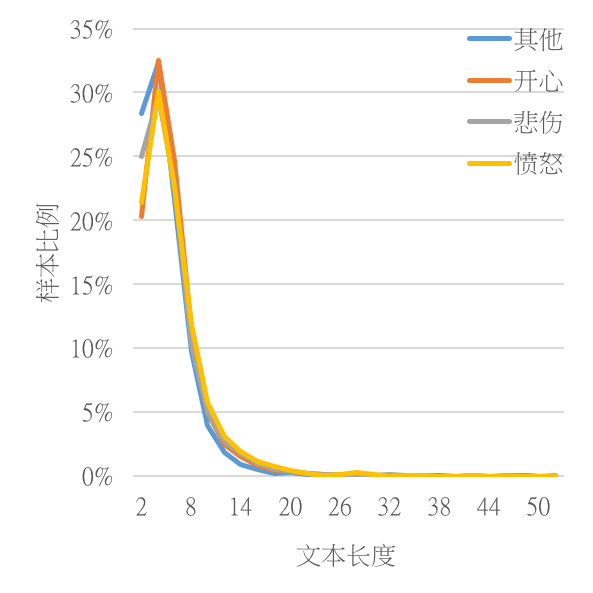
\includegraphics[height=8cm]{img/semeval2019_task3_train_0_class_len.png}}%
  %\hspace{em}%
  \subcaptionbox{第二轮\label{fig:context_emo_train_class_len_1}}
      {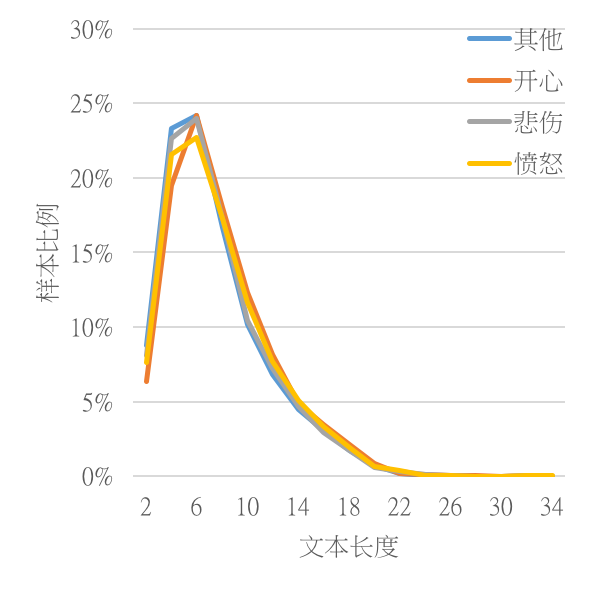
\includegraphics[height=8cm]{img/semeval2019_task3_train_1_class_len.png}}

  \end{minipage}
  \vspace{0.5cm} 

  \subcaptionbox{第三轮\label{fig:context_emo_train_class_len_2}}
      {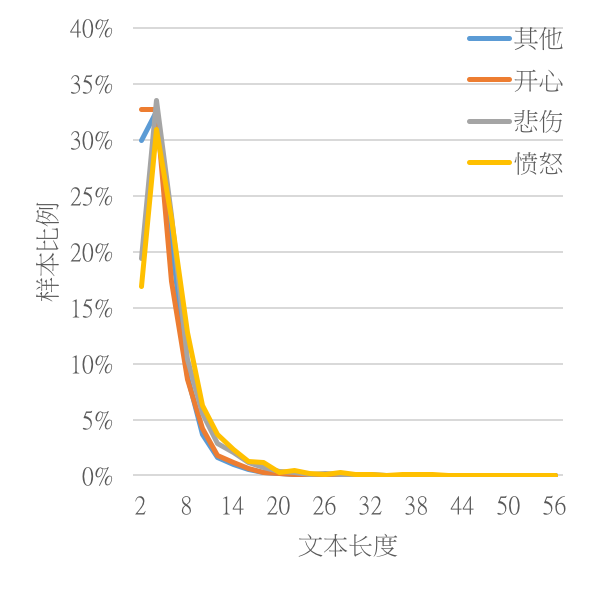
\includegraphics[height=8cm]{img/semeval2019_task3_train_2_class_len.png}}

  \caption{训练集上各情感类别的样本在每轮发言的文本长度分布}

  \label{fig:context_emo_train_class_len}
\end{figure}

\subsection{文本特征}
\label{ssec:exp_context_emo_data_text}

对于比赛中提供的数据集,比赛组织者并没有给出数据的具体来源,但经过人工观察后我们可以发现一些社交网络上常见的文本特征,其中出现频率较高的模式如下:

\begin{itemize}

\item 大量的缩略词使用,如“u”代替“you”,“y”代替“why” “im”代替“I am”。和微博以及讨论区等场景相比,可以认为在聊天场景下,用户会倾向于更快速的响应,使用缩略语减少需要输入的字符从而加快了回覆消息的速度。

\item 出现在句子最前或最后的表情符,其中包括Unicode定义表情符和由标点符号组成的表情符两类。

\item 一些在社交媒体平台上常见的、有别于正规英语的用法,如拼写错误、全大写字母的单词等,可以参考章节\ref{sec:text_preprocess}描述的例子。

\end{itemize}

\subsection{各轮发言间的情感信息}



\section{框架设计}
\label{sec:exp_context_emo_framework}

我们提出的识别系统包含了三组分类器,分别面向不同的子分类问题,并依次经过三次投票结合各组分类器的预测结果来得出最终的预测结果。第一组分类器由$N_1$个四类分类器组成,对应原问题的四个类别。第二组分类器由$N_2$个三类分类器组成,用于区分“开心”、“悲伤”和“愤怒”三类。第二组分类器由$N_3$个二类分类器组成,用于区分“其他”和不是“其他”两类(即把“开心”、“悲伤”、“愤怒”视为一个情感类别)。

对于一条待识别的微博,决策过程如下:

\begin{itemize}

\item 首先由第一组分类器内部进行多数投票得出$Label^{A}_{MV}$作为第一轮的预测结果$Label_{I}$。

\item 第二步,由第二组分类器投票进行多数投票得出预测结果$Label^{B}_{MV}$,若超过$thr_{B}$分类器投票投给$Label^{B}_{MV}$且第一轮的预测结果$Label_{I}$为“其他”以外的三种情感类别之一,则把预测结果修改为$Label^{B}_{MV}$,否则保持不变,以此得出第二轮的预测结果$Label_{II}$。

\item 最后步,由第三组分类器分别得出预测结果,若超过$thr_{C}$分类器投票投给“其他”且第二轮的预测结果$Label^{III}$不是“其他”,则把预测结果修改为“其他”,否则保持不变,以此得出第三轮的预测结果$Label_{III}$。

\end{itemize}

整个决策过程可以分成两大部分。第一部分是初步完成对第三轮发言的四分类情感识别,作为后续决策的基础,对应上述三步决策中的第一步。第二部分是基于第一部分的初步识别结果进行修正,对应上述三步决策中的后两步。第二步只关注于对“开心”、“悲伤”和“愤怒”三类的识别进行调整,因此对第一轮中结果为“其他”的样本不作改动。而第三步则是关注于对“其他”一类的召回,这受启发于样本的数据分布的不均匀。在原比赛中,组识者在最后的测试阶段虽然没有给出各个样本的真实标签,但指出了“其他”、“开心”、“悲伤”和“愤怒”四个类别在测试集上的样本比例约为88:4:4:4 ,而在训练集上的比例约为55:15:15:15 ,“其他”的样本占比在测试集上要远高于训练集。因为针对性提高“其他”一类的召回有助于提高系统在测试集上的性能。值得注意的是虽然在大部分情况下,我们无法得出应用场景的真实标签,但可以透过社会学和统计学等手段评估应用场景上各类样本的分布。而为了模型训练,我们可以人为控制训练数据上各类样本的比例。在了解到训练集和测试集上样本数据分布存在差异的情况下,提高系统对个别类别的识别倾向,其中存在其合理性。另外,虽然此框架中第二部分的设计和章节\ref{sec:exp_irony_det_framework}中的有所不同,但同样引入了可信度的概念,第二步和第三步都只在足够多个分类器给出相同结果时才对上一轮的结果进行修正。

\begin{figure}[H]
  \centering
  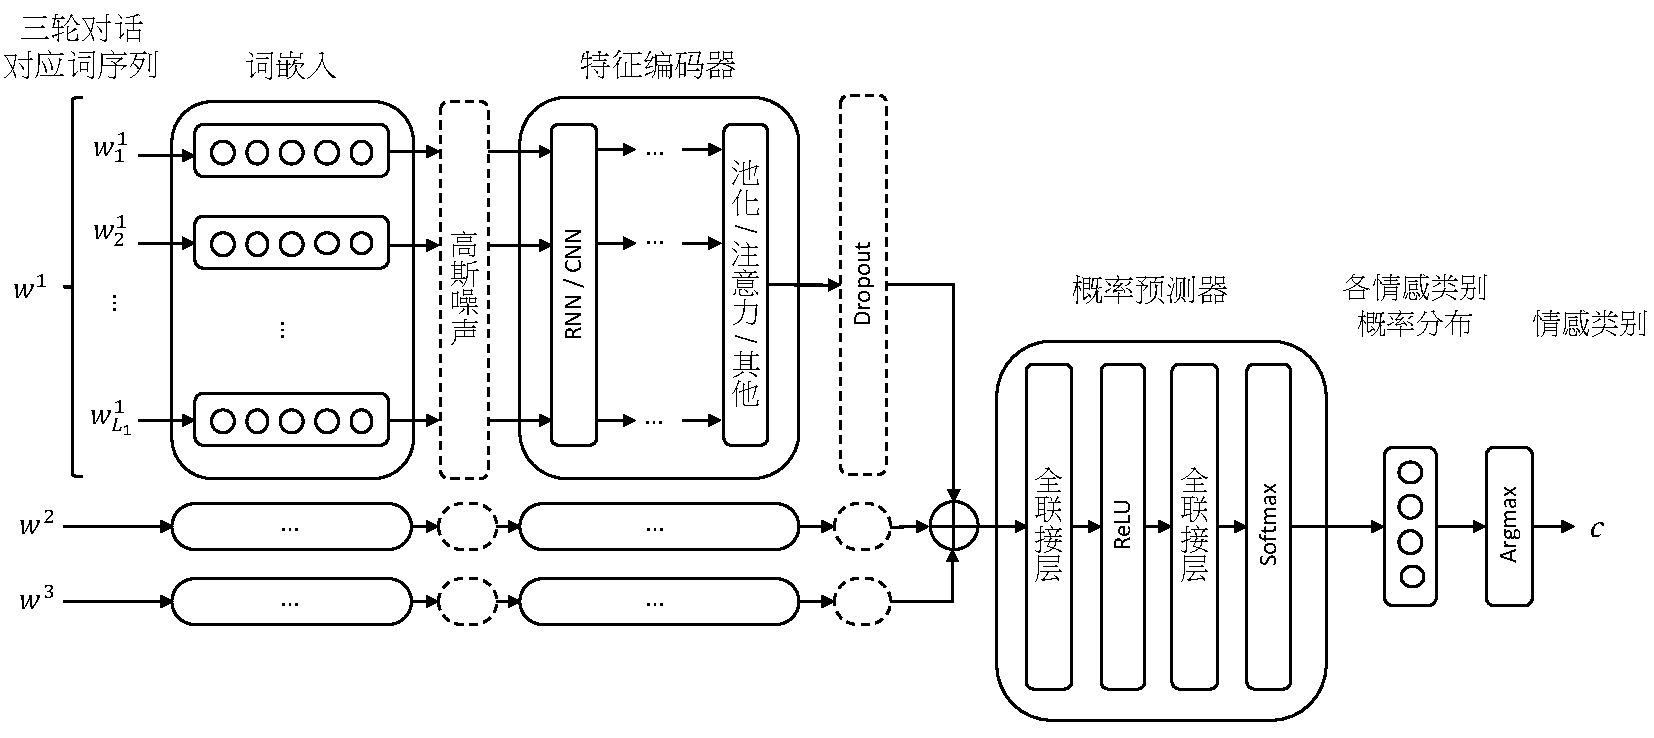
\includegraphics[width=\textwidth]{img/context_emo_cls_framework.pdf}
  \caption{三轮对话的情感识别子分类器模型框架}
  \label{fig:context_emo_cls_framework}
\end{figure}

\section{实验与分析}
\label{sec:exp_context_emo_exp}

\subsection{数据预处理}

基于我们在章节\ref{ssec:exp_context_emo_data_text}中对样本文本的观察,我们依次采取了以下数据预处理手法

\begin{itemize}

\item 全字母大写的内容在前后添加“<allcap>”和“</allcap>”,示意这一段文本可能是用户故意表示强调的内容。

\item 重复大于等次三次的标点符号以“<repeated>”示意,如“!!!”替换成序列“!”和“<repeated>”,表示“!”被多次重复以表达语气加强,同时假设重复次数不影响反讽的类型。

\item 将字母被故意重复的单词以“<elongated>”示意,如“Noooooooo”替换成序列“No”和“<elongated>”,表示“No”中某一个或多个字母被多次重复,但假设被重复的字符和重复的次数与反讽类型无关。

\item 将数字串替换成“<num>”,将电话号码替换成“<phone>”,将日期和时间分别替换成“<date>”和“<time>”,将数字百分比替换成“<percentage>”,超链接替换成“<url>”

\item 将由多个标点符号组成的表情符替换成对应的情感标签,如将“:)”替换成“<happy>”,将“:((”替换成“<sad>”。

\item 在完成以上处理后,对英文的大小写统一转换成小写。

\end{itemize}

\subsection{实验设置}

pass

\subsection{模型训练}

pass

\subsection{结果与分析}

\begin{table}[htb]
  \centering
  \begin{minipage}[t]{0.8\linewidth}
  \caption{分类器性能}
  \label{tab:exp_context_emo_0_result}
    \begin{tabularx}{\linewidth}{X|cccc}
    \toprule[1.5pt]
    & 准确率 & 正确率 & 召回率 & F1值 \\
    \hline
    CNN & \bf 0.9245 & 0.7295 & \bf 0.7584 & \bf 0.7437 \\ % f_cnn_ek_1554546621
    CNN + 注意力机制 & 0.9071 & 0.6574 & 0.7428 & 0.6975 \\ % f_cnn_ek_1554545828
    \hline
    GRU & 0.9052 & 0.7296 & 0.5481 & 0.6259 \\ % f_gru_ek_1554462561
    GRU + 注意力机制 & 0.9105 & \bf 0.7330 & 0.5974 & 0.6583 \\ % f_gru_ek_1554542220
    \hline
    BiGRU & 0.9067 & 0.6598 & 0.6923 & 0.6757 \\ % f_bgru_ek_1554465482
    BiGRU + 注意力机制 & 0.9143 & 0.7162 & 0.6947 & 0.7053 \\ % f_bgru_ek_1554524728
    \hline
    LSTM & 0.9071 & 0.6709 & 0.6911 & 0.6809 \\ % f_lstm_ek_1554465719
    LSTM + 注意力机制 & 0.8553 & 0.2994 & 0.2788 & 0.2887 \\ % f_lstm_ek_1554560984
    \hline
    BiLSTM & 0.8969 & 0.6331 & 0.6659 & 0.6491 \\ % f_blstm_ek_1554524691
    BiLSTM + 注意力机制 & 0.9092 & 0.7067 & 0.6226 & 0.6620 \\ % f_blstm_ek_1554542227
    \bottomrule[1.5pt]
    \end{tabularx}
  \end{minipage}
\end{table}

\begin{table}[htb]
  \centering
  \begin{minipage}[t]{0.8\linewidth}
  \caption{分类器性能}
  \label{tab:exp_context_emo_b_result}
    \begin{tabularx}{\linewidth}{X|cccc}
    \toprule[1.5pt]
    & 准确率 & 正确率 & 召回率 & F1值 \\
    \hline
    CNN & 0.9227 & 0.7202 & 0.7981 & \bf 0.7571 \\ % f_b_cnn_ek_1554620963
    CNN + 注意力机制 & 0.9116 & 0.6885 & 0.7572 & 0.7212 \\ % f_b_cnn_ek_1554620537
    \hline
    GRU & 0.9074 & 0.6536 & \bf 0.8233 & 0.7287 \\ % f_b_gru_ek_1554547645
    GRU + 注意力机制 & \bf 0.9230 & \bf 0.7434 & 0.7488 & 0.7461 \\ % f_b_gru_ek_1554561028
    \hline
    BiGRU & 0.9134 & 0.6824 & 0.7981 & 0.7357 \\ % f_b_bgru_ek_1554547845
    BiGRU + 注意力机制 & 0.9152 & 0.6907 & 0.7945 & 0.7390 \\ % f_b_bgru_ek_1554561013
    \hline
    LSTM & 0.9011 & 0.6347 & 0.8125 & 0.7127 \\ % f_b_lstm_ek_1554549276
    LSTM + 注意力机制 & 0.9121 & 0.6895 & 0.7608 & 0.7234 \\ % f_b_lstm_ek_1554554626
    \hline
    BiLSTM & 0.9089 & 0.6708 & 0.7788 & 0.7208 \\ % f_b_blstm_ek_1554549287
    BiLSTM + 注意力机制 & 0.9131 & 0.6814 & 0.7969 & 0.7346 \\ % f_b_blstm_ek_1554553473
    \bottomrule[1.5pt]
    \end{tabularx}
  \end{minipage}
\end{table}

\begin{table}[htb]
  \centering
  \begin{minipage}[t]{0.8\linewidth}
  \caption{分类器性能}
  \label{tab:exp_context_emo_tri_result}
    \begin{tabularx}{\linewidth}{X|cccc}
    \toprule[1.5pt]
    & 准确率 & 正确率 & 召回率 & F1值 \\
    \hline
    CNN & \bf 0.9507 & \bf 0.9454 & \bf 0.9471 & \bf 0.9462 \\ % f_tri_cnn_ek_1554620372
    CNN + 注意力机制 & 0.9351 & 0.9352 & 0.9215 & 0.9283 \\ % f_tri_cnn_ek_1554620395
    \hline
    GRU & 0.9315 & 0.9278 & 0.9142 & 0.9210 \\ % f_tri_gru_ek_1554576049
    GRU + 注意力机制 & 0.9375 & 0.9303 & 0.9252 & 0.9277 \\ % f_tri_gru_ek_1554612493
    \hline
    BiGRU & 0.9303 & 0.9212 & 0.9179 & 0.9196 \\ % f_tri_bgru_ek_1554576063
    BiGRU + 注意力机制 & 0.9339 & 0.9235 & 0.9252 & 0.9243 \\ % f_tri_bgru_ek_1554612494
    \hline
    LSTM & 0.9291 & 0.9229 & 0.9179 & 0.9204 \\ % f_tri_lstm_ek_1554575910
    LSTM + 注意力机制 & 0.9279 & 0.9180 & 0.9197 & 0.9189 \\ % f_tri_lstm_ek_1554612497
    \hline
    BiLSTM & 0.9279 & 0.9176 & 0.9142 & 0.9159 \\ % f_tri_blstm_ek_1554575896
    BiLSTM + 注意力机制 & 0.9339 & 0.9269 & 0.9252 & 0.9260 \\ % f_tri_blstm_ek_1554612490
    \bottomrule[1.5pt]
    \end{tabularx}
  \end{minipage}
\end{table}

\section{本章小结}

pass

